\documentclass{article}
\usepackage{../fasy-hw}
\usepackage{ wasysym }
\usepackage{graphicx}
\usepackage[normalem]{ulem}
\graphicspath{ {./images/} }


%% UPDATE these variables:
\renewcommand{\hwnum}{1}
\title{Computational Topology, Homework 1}
\author{Rishi Borkar}
\collab{Braeden Sopp}
\date{due: 3 February 2022}

\begin{document}

\maketitle

\input{../directions}

\nextprob{Tasks}
%\collab{n/a}

Please do the following:
\begin{enumerate}
    \item Write this homework in LaTex.  (You can use this document as a
        starting point!)  Note: if you have not used LaTex before and this is an
        issue for you, please contact me.
    \item Update your photo on D2L to be a recognizable headshot of you.
    \item Sign up for the class slack group.
    \item Fill out the course survey (found on the syllabus).
\end{enumerate}

\nextprob{}
% \collab{if applicable, update collab list}

Please read (or skim through) Eugenia Cheng’s
\href{http://eugeniacheng.com/wp-content/uploads/2017/02/cheng-proofguide.pdf}{Quick Guide for Writing
Proofs}
and describe one thing
that you already do well in your academic writing / proof writing,
and one thing that you will work on improving
throughout during this class.  You can reference additional resources, but be
sure to provide full references, either as footnotes or as a proper bibtex
citation!

\textbf{Answer:} 

During this class, I intend to work on improving the initial definitions and the assumptions that are to be made before you start the proof. I have also been told that I handwave occasionally during my proofs which I need to work on. This mainly stems from me not having an intial proper understanding of the definitions. 
However I also believe that once the inital groundwork and assumptions as setup, I do pretty well  with the rest of the proof including making use of proof by induction and contradiction.


\nextprob{}
% \collab{if applicable, update collab list}

Follow the Inkscape tutorial found here:
\url{http://tavmjong.free.fr/INKSCAPE/MANUAL/html/SoupCan.html}.
Then, make an
inkscape figure illustrating any concept that you would like.
Include the (PDF) images of both the soup can and your own figure as
floating figures in
your final write-up for this problem.  Don't forget to add a captions (and to
reference the figures!

\textbf{Answer:} 

\begin{figure}[h]
    \centering
    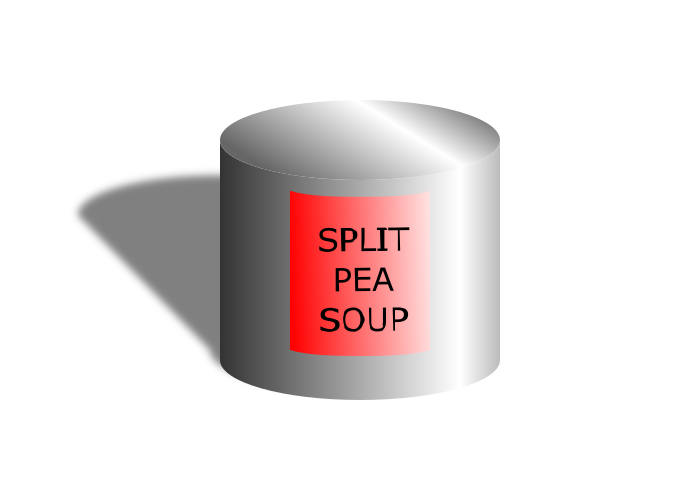
\includegraphics[width=0.60\textwidth]{can}
    \caption{A Can of Soup}
    \label{fig:A Can of Soup}~\cite{can}
\end{figure}

\begin{figure}[h]
    \centering
    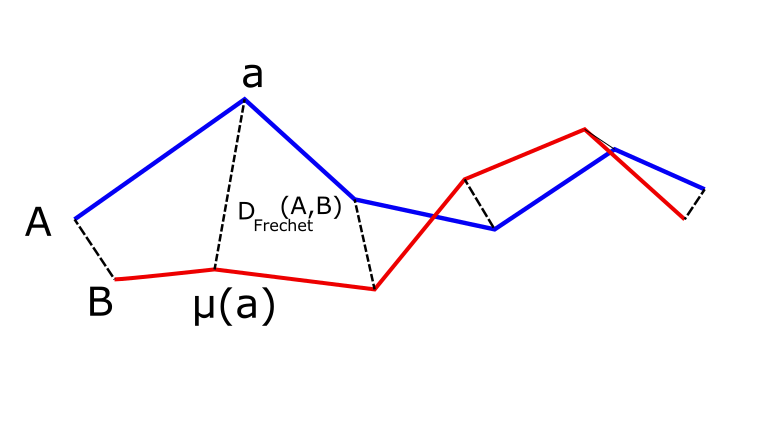
\includegraphics[width=0.60\textwidth]{bitmap}
    \caption{Frechet distance}
    \label{fig:Frechet distance}~\cite{frechet}
\end{figure}


\nextprob{}
% \collab{if applicable, update collab list}
 Watch the short \href{https://www.ayasdi.com/resources/professor-gunnar-carlsson-introduces-topological-data-analysis/}{YouTube} video.
 There is a topological
 error in the example he gives with the letter `A'.  What are the topological equivalence
classes of the letters A seen in this video?  Feel free to add additional
items to your equivalence classes for the letter `A'.  (You don't need to prove
that these are the equivalence classes, but a brief justification is expected).

\textbf{Answer:} 

All of the "A's" in the video are topologically equivalent except the below two:

\begin{figure}[h]
    \centering
    
\includegraphics[width=0.1\textwidth]{A1}
    \caption{$A_1$}
    \label{fig:$A_1$}
\end{figure}

\begin{figure}[h]
    \centering
    
\includegraphics[width=0.1\textwidth]{A2}
    \caption{$A_2$}
    \label{fig:$A_2$}
\end{figure}

Two figures are topologically equivalent if one figure can be transformed into the other by twisting and stretching, but not tearing, cutting, or gluing. Since the above two A's would require cutting or gluing to be produced from the other A's, they belong to different topological classes compared to the other A's.


\nextprob{}
% \collab{if applicable, update collab list}
Use the definition of big-O notation to prove that $f(x)=n^2 + 3n +2$ is
$O(n^2)$.

\textbf{Answer:}

$f(n)$ is $O(g(n))$ if there are positive constants C and k such that:

$f(n) \leq C g(n)$ whenever $n > k$ 
\begin{itemize}
	\item Choose k = 1
	\item Assuming $n > 1$, then
	\item $\frac{f(n)}{g(n)}$ = $\frac{n^2 + 3n + 1}{n^2} < \frac{n^2 + 3n^2 + n^2}{n^2}$ = $\frac{5n^2}{n^2} = 5$
	\item Choose C = 5. Note that $3n < 3n^2$ and $1 < n2$.
	\item Thus, $n^2 + 3n + 1$ is $O{n^2}$ because $n^2 + 3n + 1 \leq 5n^2$ whenever $n > 1$.
\end{itemize}

\nextprob{}
% \collab{if applicable, update collab list}
Let $f \colon \R \to \R$ be a function.
The function $f$ is considered continuous if for all open sets $A \subseteq \R$,
$f^{-1}(A)$ is open in $\R$, where open is defined by the standard topology on
$\R$ (so, what we normally think of as open).  Let~$c \in \R$.  Consider the
function $f_c \colon \R \to \R$ defined by $f_c(x) = c$ for all $x \in \R$. Prove
that $f_c$ is continuous.

\textbf{Answer:} 

\begin{itemize}
	\item Since $f_c \colon \R \to \R$ and  $f_c(x) = c$, which means there exists a map $x \to c$.
	\item The image of $f[\{x\}] = c$
	\item The pre-image : $f^{-1}[\{c\}] = x$
	\item Since every sub-set of a discrete topological space is open, x is open. And therefore the pre-image of $f_c(x)$ is an open set as well.
	\item Hence, $f_c$ is continuous.
\end{itemize}


\nextprob{}
\collab{Braeden Sopp}

Consider a graph $G=(V,E)$. The \emph{eccentricity} of a vertex $v \in V$ is the
maximum distance from $v$ to any other vertex in $V$. (Note: the \emph{(graph) distance} between
$a,b\in V$ is the minimum length of a path from $a$ to~$b$; the \emph{length} of
a path in an unweighted graph is the number of edges in the path). The
following algorithm computes the ecentricity of a vertex in a graph.  For the
while loop, provide the loop invariant and prove that it is the loop invariant.
In this algorithm, $Q$ is a (minimum) priority queue.

\begin{algorithm}
    \caption{Eccentricity(G,v)}
    \begin{algorithmic}[1]
        \REQUIRE a connected graph $G=(V,E)$ such that $|V| \geq 2$; a vertex $v \in V$
        \ENSURE the eccentricity of $v$
        \STATE For each vertex, add an attribute $dist$ and set it to $\infty$.
        \STATE $v.dist \gets 0$.
        \STATE Create a priority queue $Q$ of vertices, where each
                vertex $w\in V$ has priority $w.dist$.
        \STATE $maxdist \gets \infty$
        \WHILE{$Q$ is not empty}
            \STATE $w \gets $Q.pop() \COMMENT{1.5in}{Since $Q$ is a priority queue,
                                                $w.dist \leq x.dist$ for all $x \in Q$}
            \STATE $maxdist \gets w.dist$
            \FOR{each edge $(w,x) \in E$ such that $x \in Q$}
                \STATE $x.dist \gets \min \{ x.dist, w.dist +1 \} $
            \ENDFOR
        \ENDWHILE
        \RETURN $maxdist$
    \end{algorithmic}
\end{algorithm}

\textbf{Answer:} 

\textbf{Loop invariant:} At the start of each iteration, the priority queue consists only of unvisited vertices and maxdist holds the value of the eccentricity of the sub-graph made up of only the visited vertices.

\begin{figure}[h]
    \centering
    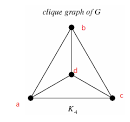
\includegraphics[width=0.25\textwidth]{clique}
    \caption{Graph}
    \label{fig:Graph}
\end{figure}


\textbf{Initialization:} At the start of the loop, the queue consists of all the vertices since none are visited and the maxdist = $\infty$ since the subgraph of visited vertices is 0


\textbf{Maintenance:} 

\begin{center}
\begin{tabular}{ |c|c|c|c|c| } 
 \hline
maxdist = $\infty$ & maxdist = 0 & maxdist = 1 & maxdist = 1  & maxdist = 1  \\ 
a = 0 &  \sout{a = 0} & \sout{a = 0} & \sout{a = 0} & \sout{a = 0} \\ 
b = $\infty$ & b = 1 & \sout{b = 1} & \sout{b = 1} & \sout{b = 1}\\ 
c = $\infty$ & c = 1 & c = 1 & \sout{c = 1} & \sout{c = 1}\\ 
d = $\infty$ & d = 1 & d = 1 & d = 1 & \sout{d = 1}\\ 
 \hline
\end{tabular}
\end{center}


\textbf{Termination:} The while-loop terminates when the queue is empty and the loop invariant gives the eccentricity of the entire graph. This is exactly the value that the algorithm should output, and which it then outputs. Therefore the algorithm is correct.


\bibliographystyle{unsrt}
\bibliography{refs}


\end{document}

